\setchapterpreamble[u]{\margintoc}
\chapter[Performance evaluation in \gls{medLabel} processes]{Performance
evaluation in \gls{medLabel} processes: standard methodology proposal and high
TBT experimental campaign}
\labch{solarmed:std}

\glsresetall % Reset glossary entries

\tldrbox{
    % This chapter presents a standard method for performance evaluation of \gls{medLabel}
    % processes, which can also be extrapolated to other thermal separation
    % processes. This method considers aspects such as instrumentation
    % requirements, process control, and the adequacy of performance metrics,
    % including uncertainty in their determination. In addition, it has been
    % developed an algorithm for the automatic identification of steady-state
    % operation, which allows to increase the reliability and robustness of
    % evaluations under variable conditions. The experimental results also show
    % that the proposed method is robust and reliable, allowing for a fair
    % comparison of \gls{medLabel} processes under different conditions.

    This chapter presents a standardized method for evaluating the performance of
    \gls{medLabel} processes, which can also be extended to other thermal
    separation technologies. The method addresses key aspects such as
    instrumentation requirements, process control, and the suitability of
    performance metrics, including the uncertainties associated with their
    determination. Additionally, an algorithm has been developed for the automatic
    detection of steady-state operation, enhancing the reliability and robustness
    of evaluations under variable conditions. Experimental results confirm that the
    proposed method is both robust and reliable, enabling fair comparisons of
    \gls{medLabel} processes across different operating scenarios.\\

    The experimentation includes the evaluation of the process at high
    \glspl{tbtLabel}. The results are analyzed using different performance
    metrics and the scale formation risk is estimated by the \fullgls{rsiLabel}.
    The results show that the \gls{medLabel} process can be operated at high
    \glspl{tbtLabel} without significant scale formation and achieve
    higher concentrations, but without significant improvements in
    thermal performance and limited concentration capacity if no changes to its
    design are made. }

\section*{Introduction}

The future of \gls{medLabel} in desalination and brine concentration
applications depends on the technical development of the process and its
integration with other
technologies~\sidecite{ghenai_performance_2021,son_pilot_2020}. The performance
of this technology and how it is evaluated plays an important role in this
development.

% Estado del arte
Although efforts have been made to propose performance metrics to evaluate
the multi-effect evaporation process, there is neither consensus in which
metrics are the most suitable~\sidecite{burgess_solar_2000} nor standards on
how to evaluate the experimental process. The only standard existing in
\gls{medLabel} is not related to performance evaluation, but to cost structures
and determinants~\sidecite{pinto_desalination_2017}. 

For the performance
evaluation of \gls{medLabel} processes, originally, the index
\fullgls{gorLabel} was used for plants operating with steam as external energy
source. In order not to be limited to steam-driven systems and to take into
account sensible heat sources, a new performance index was defined: the
\gls{prLabel}~\sidecite{mistry_entropy_2011,el-dessouky_fundamentals_2002}, which is
currently the most widely adopted for \gls{medLabel} performance evaluation
although it is constrained by using a reference enthalpy of 2326 kJ equivalent
to 1000 BTU. In \sidecite{christ_thermodynamic_2014}, a variation of this
metric called the Waste Heat Performance Ratio ($PR_{WH}$) was suggested to
account for the potential of low-grade waste heat sources. Another widespread
thermal performance metric that has been used in \gls{medLabel} is the
\fullgls{stecLabel} and its electrical equivalent, the \fullgls{seecLabel}.
% Limitaciones métricas simples
However, there are certain limitations in the aforementioned metrics that
challenge making a fair comparison between desalination systems that use
different energy sources \ie electrical and thermal\sidenote{the value of 1 kWh
electric differs from that of 1 kWh thermal in terms of their ability to
produce work, as the latter is constrained by the Carnot
efficiency~\cite{lienhard_thermodynamics_2017}}. Furthermore, the ability of
thermal energy to perform work changes with its temperature, so it is essential
to consider the quality of the thermal energy used in desalination processes.
This limitation of traditional energetic metrics was showcased in Bouma~\etal
\sidecite{bouma_metrics_2020} where they compared four different configurations
of \gls{medLabel} plants: a low temperature \gls{medLabel} configuration
(LT-MED), a \gls{medLabel} unit incorporating Thermal Vapor Compression
(MED-TVC), a \gls{medLabel} unit using nanofiltration (NF-LT-MED) for feedwater
pretreatment, and a combination of TVC and nanofiltration. Although the
\gls{stecLabel} values favored the use of TVC, a more rigorous ---exergetic---
analysis revealed that the most efficient systems were those that used lower
temperature heat sources (LT-MED and NF-LT-MED).

%Furthermore, each energy type possesses different thermodynamic or economic
%values, further complicating the evaluation process. It is important to note
%that the value of 1 kWh electric differs from that of 1 kWh thermal in terms
%of their ability to produce work, as the latter is constrained by the Carnot
%efficiency. Consequently, a system that excels according to one metric may do
%so at the expense of the other, and even assessing the same system under
%different conditions can prove difficult. Secondly, the quality of thermal
%energy is not uniform, and its evaluation depends on its temperature-dependent
%thermodynamic properties~\sidecite{darwish_multi-effect_2006}. As the temperature
%of thermal energy rises, its ability to perform work or its availability
%increases, indicating higher exergy or quality. Hence, when assessing the
%practical applications of an \gls{medLabel} system, the quality of thermal energy
%employed becomes a critical factor. 

% Estado del arte de análisis exergéticos. Thermal energy is not a homogeneous
%form of energy, and its quality is determined by its thermodynamic properties,
%which are temperature-dependent~\sidecite{darwishMultieffectBoilingSystems2006}.
%As the temperature of thermal energy increases, so does its ability to do work
%or availability, which is reflected in its higher exergy or quality.
%Therefore, the quality of thermal energy used in an \gls{medLabel} system is a crucial
%factor in evaluating its performance in practical applications. This
%limitation of traditional metrics was showcased in
%\cite{boumaMetricsMatterAccurately2020}, where four \gls{medLabel} plants configurations
%were compared: a basic configuration, one that included Thermal Vapor
%Compression (TVC), one where the feedwater was pretreated with nanofiltration
%(NF) and a combination of both. Even though STEC figures favored the use of
%TVC an exergetic analysis reveals that SEXC values actually fall towards the
%basic \gls{medLabel} or MED-NF. 

Some authors have carried out exergy analysis to overcome the limitations
aforementioned of energy performance metrics. Darwish~\etal
~\sidecite{darwish_multieffect_2006} proposed two new metrics: Specific Fuel
Energy and Equivalent Specific Work. The first compares the energy used for the
desalination process that could otherwise be used for energy generation in a
turbine for which it was assumed a value for the efficiency of the power plant.
The second sets the work potential of the extracted steam as a baseline,
considering the desalination plant separation efficiency and adding the energy
consumption for pumping. The problem of this study is that it is limited to
cogeneration schemes (joint electricity and water production) and would not be
useful in the case of desalination with low-temperature sources. Shahzad et
al.~\sidecite{shahzad_standard_2019} developed an approach based on the second
law of thermodynamics, which is also useful only for cogeneration schemes. They
proposed a common metric called the Standard Universal Performance Ratio to
compare desalination processes using different kinds of energy, which is based
on conversion of different types and grades of energies to standard primary
energy. In this case, conversion factors were proposed to convert the derived
energy input to the standard primary energy. Other authors have performed
exergy analyses for stand-alone desalination processes, as is the case of
Lienhard~\etal~\sidecite{lienhard_thermodynamics_2017} and Brogioli et
al.~\sidecite{brogioli_thermodynamic_2018}, who considered desalination
processes as a black box and the ideal work or the thermodynamic limit for the
separation of dissolved salts in seawater as the Carnot work.

The problem with the exergy analyses is that they are more complex
~\sidecite{spiegler_energetics_2001} due to the need to consider several aspects
not present in simple energetic metrics: definition of dead state and control
volume~\sidecite{sharqawy_exergy_2011}, chemical exergy modeling of seawater
~\sidecite{sharqawy_formulation_2010,mistry_effect_2012} and minimum energy
reference (least and minimum work of separation)
~\sidecite{mistry_generalized_2013,thiel_energy_2015}. Probably because of
their complexity, they have not been widespread in the performance evaluation
of practical setups. Also, none of the works published so far in the scientific
literature addresses specifically the exergetic evaluation when using
non-conventional energy sources such as waste heat.
%The practical evaluation of waste heat sources using the exergy alternative is
%another aspect that has yet to be resolved in the literature. % An equivalent
%approach to the one proposed by Christ~\etal~\sidecite{christ_thermodynamic_2014}
%is applied to exergy analysis, in order to come with new metrics that allow to
%make fair assessments of this kind of energy sources.


%However, this complexity has been reduced by the work of various authors in
%the last decade
%\cite{sharqawy_exergy_2011,mistry_entropy_2011,mistry_generalized_2013,thiel_energy_2015,lienhard_thermodynamics_2017}.
%Among these ones, Sharqawi~\etal
%\cite{sharqawy_formulation_2010,sharqawy_thermophysical_2010} included a
%chemical exergy term accounting for the composition of real seawater. In
%addition, experts such as Mistry and Lienhard have extensively covered various
%aspects of the exergy analyses and their application in thermal desalination.
%Their contributions include seawater chemical exergy modeling
%\cite{mistry_effect_2012} and the analysis of the least work of separation
%\cite{mistry_generalized_2013}. A compilation of all these valuable works can
%be found in~\sidecite{lienhard_thermodynamics_2017}.

% Como estaba PP: Although the efforts of the authors to include the use of
% exergetic evaluations it is still limited to academic works and they have not
% been used by the thermal desalination industry so far. On the other hand,
% there is still a gap in the use of waste heat as thermal energy source.

% Comentar alguna estandarización en otros procesos. Remarcar importancia /
% necesidad
Two important requirements for an accurate and reliable performance assessment
are the steady state identification and the uncertainty of both the direct
measurement and that associated with the performance metric determination. With
respect to the former, it is highly recommended to use automatic procedures that
increase the reliability of the measurements. The steady state evaluation
carried out manually so far by qualified operators
~\sidecite{valenzuela_optical_2014,prahl_protocol_2018,bayon_development_2019},
leads to high time consumption and full dependence on the operators' attention,
leading to potential unreliable identifications. With respect to the latter, it
allows for a more comprehensive and nuanced approach to performance evaluation,
since it increases the robustness of the evaluation while providing information
on the reliability of the results. Neither of these two aspects have yet been
addressed in the performance assessment of thermal desalination plants. There is
a gap in the establishment of standard methodologies that include all the
necessary requirements for the reliable assessment of the performance of thermal
desalination processes. This chapter aims to address this gap by proposing a
method with potential for a broader application in other thermal desalination
processes. The method is applied and validated in the \gls{medLabel}-\gls{psaLabel}
plant as part of a high \gls{tbtLabel} experimental campaign.

%Recently, different regulations and methodology proposals have been set to
%standardize certain procedures for other technologies under the umbrella of
%projects funded by the European Commission and it is time to start doing that
%for thermal desalination. One common feature between thermal desalination and
%parabolic-through collectors is that performance tests must be evaluated in
%steady state conditions. This requirement can be achieved manually by
%qualified operators, but  %An automatic procedure is proposed in this paper
%with the aim of being used in other similar procedures as well.


% Contribuciones In this work a novel comprehensive methodology for the
%performance evaluation of \gls{medLabel} processes in practical settings is proposed,
%covering all practical aspects of such evaluation and validated in an
%experimental \gls{medLabel} plant. The objective is to serve as the base for the eventual
%standardization of \gls{medLabel} processes evaluation applicable to other thermal
%desalination processes. 

% that includes all the practical aspects of a reliable
% performance evaluation of \gls{medLabel} processes\sidenote{}. 
% Concretely, this standard method includes: instrumentation requirements
% supported by a sensitivity analysis, control system specifications, exergy
% analysis for all kinds of energy sources, an algorithm for the steady-state
% automatic detection and the uncertainty of the direct measurement and the one
% associated with the performance metric determination. Results and discussion on
% its successful application in a pilot \gls{medLabel} plant located on the
% Plataforma Solar de Almería

% (PSA) are presented.

%a critical but often neglected factor, the uncertainty of both, the direct
%measurement and that associated with the performance metric determination. It
%increases the robustness of the evaluation while providing a more realistic
%understanding of the process, allowing for a more comprehensive and nuanced
%approach to performance evaluation. 

\subsubsection{Evaluation at high \glsentrylong{tbtLabel}}

%\annotation{Performance of a thermal separator}{
The performance of a thermal process, such as \gls{medLabel}, is dictated by the
Carnot cycle~\sidecite{brogioli_thermodynamic_2018}, which sets the theoretical
maximum efficiency for any heat engine. The efficiency of the Carnot cycle is
limited by the temperature difference between the hot and cold sinks, which
determine the amount of thermal energy that can be converted into useful
(separation) work.

An approach to bring the \gls{medLabel} closer to its thermodynamic limit can be
achieved by raising the \fullgls{tbtLabel} (from 70 to 80--90$^\circ$C), which
allows to increase the number of effects~\cite{mistry_improved_2013} while
maintaining an optimal temperature drop across them
(\textit{pinch})\sidenote[][*-3]{With limitations, as in each effect a
considerable amount of exergy is destroyed and a minimum pinch is required}.
This leads to an improvement in the thermal performance of traditional
desalination applications and an increase in the concentration factors
achievable~\sidecite{zaragoza_coupling_2022}.

\annotation{High \gls{tbtLabel} does not mean high heat source temperature}{
    \gls{medLabel}-\gls{tvcLabel} plants even when operating at low
    \gls{tbtLabel} require motive steam at \textit{high} temperatures
    (120--150$^\circ$C)~\cite{palenzuela_concentrating_2015}. However, the
    extension of the \gls{medLabel} process to higher \gls{tbtLabel} values in
    the range of 80--90$^\circ$C still requires relatively low temperature heat
    (<100$^\circ$C), so it can still be considered low-temperature and
    compatible with low-grade waste heat sources. 
}

In practice, the \gls{tbtLabel} in the \gls{medLabel} system is limited to
70$^\circ$C, since higher \glspl{tbtLabel} increase the risk of precipitation of
divalent ions, which tend to form incrustations on the heat exchange surfaces.
These deposits reduce heat transfer efficiency, as extensively analyzed
by Glade~\etal~\sidecite{glade_scale_2010,kromer_scale_2015}. 

\annotation{Ryznar Stability Index (RSI)}{The \gls{rsiLabel} is an
  empirical indicator used in water chemistry to predict the tendency of water
  to form scale (calcium carbonate deposits) or to cause corrosion. It is based
  on the Langelier Saturation Index (LSI) but is formulated to better correlate
  with observed scaling and corrosion behavior~\cite{ryznar_new_1944}. It is
  defined as:\\ 
  
    \begin{minipage}{\textwidth}
        \centering
        $RSI = 2 pH_s - pH$,\\
    \end{minipage}
  
  where $pH$ is the measured pH of the
  water sample and $pH_s$ is the pH at which the water is saturated with calcium
  carbonate (CaCO$_3$).}

\reffig{solarmed:std:rsi-seawater} shows the \gls{rsiLabel} of seawater at
different temperatures and concentrations, where the background surface color
represents the \gls{rsiLabel}. For un-treated feedwater this risk of
precipitation is present at almost any temperature due to its composition
(\gls{rsiLabel} below 4, see \reftab{solarmed:rsi}). This situation can be
attenuated either by the use of an anti-scalant, or by treating the feedwater to
remove the divalent ions. One promising option to achieve the latter is to use
selective nanofiltration membranes~\sidecite[*-5]{schafer_nanofiltration_2021}.
A nanofiltration pretreatment can be used to selectively remove the divalent
ions while leaving relatively unaffected the components to be separated in the
\gls{medLabel} process, \ie NaCl. This allows the operation of \gls{medLabel}
processes at higher \glspl{tbtLabel} or higher feed concentration.

\begin{marginfigure}[*-5]
    \includegraphics[]{scaling_analysis_RSI_sw.png}
    \caption{\gls{rsiLabel} of seawater at different temperatures and concentrations}
    \labfig{solarmed:std:rsi-seawater}
\end{marginfigure}

This second feature potentially enables hybrid systems combining two separation phases \eg:
an initial \gls{roLabel} stage for traditional seawater desalination followed by
a \gls{medLabel} brine concentrator that tolerates higher feed concentrations.


\bigskip

The chapter is structured as follows. First, in \refsec{solarmed:std:process}, a
process analysis focused on performance evaluation is presented to clearly
define the evaluation scope as well as the process inputs and outputs. Then, in
\refsec{solarmed:std:metrics}, the performance metrics are introduced, including
separation, energetic, and exergetic criteria.
\refsec{solarmed:std:instrumentation} describes the system instrumentation,
covering \glspl{kpvLabel}, instrumentation requirements, and the uncertainty
determination for both direct measurements and derived metrics.
\refsec{solarmed:std:control-monitoring} presents the proposed steady-state
identification algorithm for stable operation monitoring, together with the
control strategies to be implemented. Finally, in \refsec{solarmed:std:results},
the proposed methodology is applied to a case study ---an experimental campaign
at the \gls{medLabel}-\gls{psaLabel} plant--- to experimentally characterize the
system under high \glspl{tbtLabel}. The results of this high-\gls{tbtLabel}
operation are also analyzed in this section.

\begin{margintable}[*-7]
\caption{\fullgls{rsiLabel} values and their interpretation in terms of scaling and corrosion risk~\cite{ryznar_new_1944}.}
\labtab{solarmed:rsi}
\resizebox{\linewidth}{!}{%
\begin{tabular}{cl}
    \toprule
    RSI > 9 & Severe corrosion \\
    7.5 < RSI < 9 & Heavy corrosion \\
    7 < RSI < 7.5 & Significant corrosion \\
    6 < RSI < 7 & Stable water \\
    5 < RSI < 6 & Moderate to light scaling \\
    4 < RSI < 5 & Severe scaling \\
    \bottomrule
\end{tabular}
}
\end{margintable}

%===================================
%===================================
\section{Process analysis}
\labsec{solarmed:std:process}

Metrics are defined based on some criteria, and this criteria is of paramount
importance because resources and efforts are invested in optimizing the process
in its direction. In order to adequately define these criteria, it is important
to have an overall perspective of the process: defining its inputs and useful
outputs ---from a qualitative point of view--- as well as a clear delineation of
the scope of the evaluation. 

%It is as if an already built system is provided, so
%decision over its design parameters and energy source conditions is not an
% available degree of freedom, only optimization in its operational variables. 

Metrics can be related either to the operation or to the design of the
system\sidenote[]{\eg a design metric would be the specific
area~\cite{el-dessouky_fundamentals_2002}}. In terms of scope, they can span
from primary energy sources~\sidecite{bouma_metrics_2020} or the isolated
\gls{medLabel} process. This chapter focuses on the \textbf{operation} of an
\textbf{isolated} \gls{medLabel} system. Additionally, for the determination of
the performance metrics, the following aspects are considered:

\textbf{Application}. Two applications are distinguished: 
\begin{itemize}
    \item \textbf{Seawater desalination}. The objective is to obtain fresh
    water. The level of separation achieved is a secondary (not useful) output.

    \item \textbf{Brine concentration}. The objective is to extract resources
    from the brine in order to valorize it. Here, the level of separation is a
    crucial factor to consider.
\end{itemize}

\textbf{External heat source type}. Two types of external heat sources are
distinguished\sidenote{The use of electrical energy will always be desired to
be minimized, so the distinction is not needed.}:
\begin{itemize}
    \item \textbf{Process heat}. Process heat is the heat utilized by a system
    and its associated costs are related to the amount of energy consumed.
    
    \item \textbf{Waste heat}. Waste heat is the heat utilized by a system that
    would otherwise be lost to the environment. It has no associated costs to
    the amount of heat used, though there are other costs associated with its
    use\sidenote{\eg a less efficient system will require a larger heat
    exchanger area to extract more energy from the waste heat source, leading to
    increased system
    costs}~\sidecite{mistry_economicsbased_2013,christ_technoeconomic_2017}.
    Here the goal is to maximize the amount of product by maximizing the
    utilization of the waste
    source~\sidecite{christ_thermodynamic_2014,christ_application_2015,christ_boosted_2015}.
\end{itemize}

\annotation{Process heat \textit{vs} waste heat take on efficiency}{
    In a process heat driven system, between two plants that produce the same
    amount of useful product, the most efficient one is the one that uses the
    least external heat to do so, whereas in a waste heat driven system, the
    two plants would be considered as efficient since the unused heat would be
    \textit{wasted} to the environment. A more intuitive definition would be:\\
    
    Given two plants that consume the same waste heat, the most efficient one is
    the one that produces the most product with that available heat. }

% Volumen de control
Based on the above considerations, \reffig{solarmed:std:control-volume} shows
the control volume of the \gls{medLabel} process with the inputs and outputs
used for the definition of the performance metrics. From left to right, seawater
(including cooling water, $c$, and feed, $f$) enters the control volume at the
seawater intake conditions ($T_{c,in}$). The cooling water is rejected at
$T_{c,out}$. On the right side, the distillate and the brine are discharged from
the \gls{medLabel} system at temperatures $T_{d,out}$ and $T_{b,out}$ and mass
fractions $w_d$ and $w_b$, respectively. The temperatures of all these outlet
streams, from a qualitative (\ie exergetic) point of view, are useless and thus
considered to be at $T_0$ when leaving the control volume\sidenote{It is heat
that is lost to the environment, and thus no additional work can be feasiblly
extracted from these streams}.

\begin{figure}
    \includegraphics[width=.8\textwidth]{solarmed-control-volume.png}
    \caption{Inputs and outputs variables in an \gls{medLabel} process. The dash line delimits the control volume}
    \labfig{solarmed:std:control-volume}
\end{figure}

From top to bottom, the energy sources for the system are depicted. Electrical
work is depicted as $\dot{W}_{electrical}$ and includes pumping, vacuum
system, and feed water pretreatment, among others. The heat source is
represented by the subscript ($s$) and as shown in the figure, it enters the
\gls{medLabel} plant at $T_{s,in}$ and leaves it at $T_{s,out}$ after releasing
part of its energy. When leaving the control volume, $T_{s,out}$ value depends
on the type of heat source:

\begin{itemize}
    \item Process heat (PH). The value of $T_{s,out}$ does not change. In case
    steam is used as heat source, the primary energy driver is the latent heat
    of phase change and $T_{s,out}$ is usually similar to or equal to
    $T_{s,in}$. In case a sensible heat source is used, the driving force is the
    temperature difference and $T_{s,out}$ is between $T_{s,in}$ and $T_0$.

    \item Waste heat source (WH). In this case, $T_{s,out}$ is considered to leave
    at the sink conditions ($T_0$) since this heat is not reused but lost to the
    environment.
\end{itemize}
    

%===================================
%===================================
\section{Performance metrics}
\labsec{solarmed:std:metrics}

A performance metric is a quantitative measure used to evaluate the
effectiveness or efficiency of a system. It provides objective information that
can be used to monitor progress, identify areas for improvement, and inform
decision making. A metrics division in three categories is proposed:
separation, energetic, and exergetic metrics. A detailed description of each of
them within each category is presented below.

%================================
\subsection{Separation metrics}
\labsec{solarmed:std:metrics:separation}

\textbf{Recovery Ratio}. The \fullgls{rrLabel} represents the flow ratio of unit
of distillate produced per unit of feed and is very useful in seawater brine
concentration applications~\sidecite{jones_state_2019}. It is related to
electricity consumption, since the lower the \gls{rrLabel} the higher the feed
pumping needs are for the same distillate
production~\sidecite{palenzuela_concentrating_2015}. It is determined as
follows:

\begin{equation}\labeq{RR}
  RR=\frac{\dot{m}_d}{\dot{m}_{f}} \times 100 \: \left[\%\right],
\end{equation}

where $\dot{m}_d$ is the mass flow rate of distillate and $\dot{m}_f$ is the
feedwater mass flow rate, both in kg/s.

\textbf{Concentration Factor}. An equivalent metric is the concentration factor,
which accounts for how many times the brine is concentrated with respect to the
feed concentration:
\begin{equation}
    CF=\frac{w_b}{w_f}=\frac{\dot{m}_f}{\dot{m}_f-\dot{m}_d} \: \left[-\right],
\end{equation}

where $w_b$ is the brine concentration and $w_f$ is the feedwater
concentration, both in g/kg. \\

\textbf{Reconcentration Index}. Apart from the already known previous metrics, a
new one is proposed in this work that can be useful for seawater brine
concentration applications. This metric is called \gls{riLabel}, and it
allows to determine how close the separation achieved (\gls{rrLabel}) is to the
theoretical maximum recovery ratio ($RR_{max}$). It is defined as:

\begin{equation}
    RI=RR/RR_{max} \: \left[-\right],
\end{equation}

where $RR_{max}$ is calculated as follows~\sidecite{thiel_energy_2015}:
\begin{equation}\labeq{rr_max}
    RR_{max}=w_{w,f} \left( 1- \frac{b_{NaCl,f}}{b_{NaCl,sat}} \right) \times 100 \: \left[\%\right],
\end{equation}

% = w_{w,f} \left( 1-\frac{\gamma_{\pm NaCl,sat} b_{NaCl,f}}{\sqrt{K_{sp}}}
% \right)

where $w_{w,f}$ is the water mass fraction in the feed (which is $1-w_{sol,f}$,
where $w_{sol,f}$ is the mass fraction of the solutes in the feed) and
$b_{NaCl,f}$ is the molality of sodium chloride in the feed, in
mol$_{NaCl}$/kg$_w$ (both can be obtained from a feedwater chemical analysis).
On the other hand, $b_{NaCl,sat}$ is the molality of sodium chloride at
saturation conditions\sidenote{sodium chloride is the only solute considered, as
it sets the concentration limit being the solute in seawater with the highest
concentration and the greatest solubility~\cite{thiel_energy_2015}} (see
\nrefsec{appendix:rr_max} for more details of its estimation).

% which is set to $6.01 \: mol/kg$ (it changes with temperature and pressure).

% Also can be calculated in terms of the mean molal activity coefficient at saturation $\gamma_{\pm,Nacl,sat}$ and the solubility product $K_{sp}$.

%================================
\subsection{Energetic metrics}
\labsec{solarmed:std:metrics:energetic}

% Introducción explicando que son métricas basadas en la primera ley de la
% termodinámica
The energetic metrics are metrics that consider only the first law of
thermodynamics (\ie quantity). They are: \fullgls{gorLabel}, \fullgls{stecLabel}, and \fullgls{seecLabel} and are described in the following.

% GOR
\textbf{Gain Output Ratio}. Regarding the \gls{gorLabel}, a universal definition of this metric that avoids
the limitations of some of the commonly used definitions mentioned\sidenote{Limited to steam or 1000 BTU as arbitrary conversion
factor} is the ratio between the energy in the form of latent heat required to
vaporize all the distillate produced and the external thermal energy
contributed to the system (\refeq{GOR})~\sidecite{lienhardv_solar_2012}.

%\begin{equation}\labeq{GOR}
    %GOR = \frac{\dot{m_d}}{\dot{m_{s}}} \approx \left.
    %\left(1-\frac{w_{f}}{w_{b}}\right) \cdot \frac{\dot{m}_{f}}{\dot{m}_{d}}
    %\right|_{ w_{d} \rightarrow 0 }\: \left[-\right],
%\end{equation}

\begin{equation}\labeq{GOR}
     GOR = \frac{\dot{m}_{d} · \Delta h_{avg}} {\dot{Q}_{in}} 
\end{equation}
% \begin{equation}\labeq{GOR} GOR = \frac{\dot{m}_{d} · \Delta h_{v,avg}}
%     {\dot{m}_s · \Delta h_s} = \frac{\dot{m}_{d} (h_{v,1} - h_{v,c}})
%     {\dot{m}_s · \Delta h_s} \end{equation}

where $\Delta h_{avg}$ is the latent heat of vaporization at the average vapor
temperature between the first effect and the last effect, in KJ/kg, 
%$\dot{m_s}$ is the mass flow rate of the external energy source supplied in
%the first effect, in kg/s 
and $\dot{Q}_{in}$ is the external thermal energy consumption required to drive
the process, in kW. In case process heat is used, it is determined by
$\dot{m}_s$ (mass flow rate of the external energy source supplied in the first
effect, in kg/s) and $\Delta h_s$, which can be calculated as
$h_{s,in}-h_{s,out}$ (in case of sensible heat) or as
$h_{s,sat.vap}-h_{s,sat.liq}$  (in case of latent heat of phase change at
saturation conditions from vapor to liquid at temperature $T_{s,in}$).

 

%The PR is defined as the ratio between the distillate produced and the thermal
%energy supplied to the process, normalized to 2326 kJ/kg, which is the latent
%heat of vaporization of pure water at 73 $^{\circ}$C. 

% PR \begin{equation}\labeq{PR} PR = \frac{\dot{m_d}} {\dot{m_s}}
%\frac{\Delta h_{ref}} {\Delta h_{s}} \: \left[-\right], \end{equation}

% =  \Bigg\{ \begin{matrix} \frac{\dot{m_d}}{\dot{m_s}} \frac{2326 kJ}
% {c_{p,s}·(T_{s,in} - T_{s,out})} & (sensible\;source)\\
% \frac{\dot{m_d}}{\dot{m_s}} \frac{2326 kJ}
% {\lambda_{s,sat.vap}-\lambda_{s,sat.liq}}& (latent\;source) \end{matrix}
% where $\Delta h_{ref}$ is a reference enthalpy of 2326 kJ equivalent to 1000
% BTU and $\Delta h_{s}$ is the enthalpy variation of the energy source.
% Depending on the heat source type $\Delta h_s$ can be calculated as $h_{s,in}
% - h_{s,out}$ (sensible heat) or as $h_{s,sat.vap}-h_{s,sat.liq}$ (latent heat
% of phase change at saturation conditions from vapour to liquid at temperature
% $T_{s,in}$). By definition, $GOR$ and $PR$ are equivalent at 73 $^{\circ}$C.
% For temperatures higher than 73 $^{\circ}$C, the $PR$ is overestimated and
% the opposite happens for temperatures below this value. The magnitude of this
% difference can be up to 6\% for a temperature range of 10-120~$^\circ$C.

% PR_WH
In case waste heat is used as external thermal energy source for the \gls{medLabel}
system, $\dot{Q}_{in}$ is determined with ${\dot{m_s}}$ and ${\Delta h}$ but
referred to the lowest temperature of the system ($T_{c,in}$). 

\textbf{Specific Thermal Energy Consumption}. Another performance index widely
used in thermal desalination is the \fullgls{stecLabel}. For desalination
applications, it is defined as the input heat to the system per unit of product
(distillate). If process heat is used, this index has units of energy per
fraction of volume and its expression is shown in \refeq{STEC}.
%$\left( \frac{kWh_{th}}{m^{3}} \right)$.

\begin{equation}\labeq{STEC}
STEC = \frac{\dot{m}_{s}·(h_{s,in}-h_{s,out})}{\dot{m}_{d}} · \rho_{d}· \frac{1\:\mathrm{kWh}}{3600\:\mathrm{kJ}} \: \left[ \frac{\mathrm{kWh}_{\mathrm{th}}}{\mathrm{m}^{3}} \right].
\end{equation}

For brine concentration applications, it is named as $STEC_{bc}$ and it is
determined as the energy required (in kJ) per unit of feed (in kg) (\ie
$\dot{m}_f$ in the denominator)~\sidecite{chen_zero_2021}.

Both \gls{stecLabel} and \gls{gorLabel} are equivalent and are related via \refeq{PR_STEC}.

\begin{equation}\labeq{PR_STEC}
    STEC = \frac{2326 \: \mathrm{kJ/kg}}{GOR} · \rho_d · \frac{1 \: \mathrm{kWh}}{3600 \: \mathrm{kJ}},
\end{equation}

where $\rho_d$ is the density of the distillate in $\mathrm{kg}/\mathrm{m^3}$. 

For the cases in which waste heat source is used as energy source, a variation
of the \gls{stecLabel} is proposed: the waste heat \gls{stecLabel}
($STEC_{wh}$). For desalination applications, it is determined as follows:
\begin{equation}\labeq{STEC_WH}
STEC_{wh} = \frac{\dot{m}_s · (h_{s,in}-h_{c,in})}{\dot{m}_{d}} · \rho_{d}· \frac{1\:\mathrm{kWh}}{3600\:\mathrm{kJ}} \: \left[ \frac{\mathrm{kWh}_{\mathrm{th}}}{\mathrm{m}^{3}} \right].
\end{equation}

As before, for brine concentration applications, $\dot{m}_d$ would be replaced
by $\dot{m}_f$ in the denominator.

\textbf{Specific Electrical Energy Consumption}. Another important index in
desalination is the \fullgls{seecLabel}, which represents the total electrical
consumption of the plant per unit of distillate water produced. These are the
subsystems that should be considered:

\begin{itemize}
    \item $J_s$. External heat source pumping (if any)
    \item $J_f$. Feed pumping
    \item $J_c$. Cooling
    \item $J_d$, $J_b$. Discharge extractions
    \item $J_{vacuum}$. Vacuum system
    \item $J_{aux}$. Auxiliary consumptions. Represents any additional power
    that the system may require to function (\eg, electrical consumption for
    feedwater pretreatment such as nanofiltration)
\end{itemize}

For desalination applications, the following equation is used for the
calculation of this metric:

\begin{equation}\labeq{SEEC}
SEEC = \frac{\sum\limits_{i=1}^N(J_{i})}{\dot{m}_{d}} \: \left[ \frac{\mathrm{kWh}_{\mathrm{e}}}{\mathrm{m}^{3}} \right],
\end{equation}

where $J_{i}$ is the electrical consumption of the $i_{th}$ subsystem. In the
case of brine concentration applications, the index is called $SEEC_{bc}$ and
the denominator would be replaced by $\dot{m}_f$. 

%================================
\subsection{Exergetic metrics}
\labsec{solarmed:std:metrics:exergetic}

Exergy is the maximum amount of work achievable when a system is brought into
equilibrium from its initial state to a reference state (known as the dead
state and represented by the subscript ``$0$")
\cite{sharqawy_exergy_2011,bejan_advanced_2016}. This reference state is
usually established for desalination applications as the seawater intake
temperature ($T_{c,in}$). In contrast to the energetic metrics, it considers
not only the first law of thermodynamics (quantity), but also the second law
(quality). 
%Different to the energetic metrics, it takes into consideration not only the
%First Law of Thermodynamics (quantity) but also the Second Law of
%Thermodynamics (quality). There are several aspects of exergy analysis that
%need to be firstly considered in order to be able to make fair exergy 

% eta II
\textbf{Second law efficiency}. The most widespread exergetic metric is the second law efficiency
($\eta_{II}$)~\sidecite{lienhard_thermodynamics_2017}, which accounts for
irreversible losses within a system. It is calculated as the ratio of the
useful exergy output of a system ($\dot{E}x_{out,useful}$) to the exergy input
given to the system ($\dot{E}x_{in}$) (a further explanation of how to
determine the different exergy flows can be found in \nrefsec{appendix:exergy}):

\begin{equation}
    \eta_{II} = \frac{ \dot{E}x_{out,useful} }{ \dot{E}x_{in} } \times 100 \: [\mathrm{\%}].
\end{equation}

Considering exergy losses, which are the sum of the exergy destroyed in each
individual component ($\dot{E}x_{destroyed}$) and exergy losses due to
discharge streams in disequilibrium to the environment ($\dot{E}x_{streams}$),
the previous equation can be written as follows:

\begin{equation}\labeq{eta}
    \eta_{II} = 1 - \frac{\dot{E}x_{destroyed}+\dot{E}x_{streams}}{\dot{E}x_{in}} \times 100 \: [\%].
\end{equation}

% SEXC
\textbf{Specific Exergy Consumption}. Another useful metric is the
\gls{sexcLabel}, which was firstly referenced as specific consumed available
energy in \sidecite{darwish_multieffect_2006}. Similarly to \gls{seecLabel} and
\gls{stecLabel}, it accounts for the exergy input to the system per unit of
distillate produced (\refeq{SEXC}) and it is determined as
follows~\sidecite{bouma_metrics_2020}:

\begin{equation}\labeq{SEXC}
    SEXC = \frac{\dot{E}x_{in}}{\dot{{m}_d}} \: \left[ \frac{\mathrm{kWh}_{\mathrm{ex}}}{\mathrm{m}^3} \right].
\end{equation}

It is important to note that the terms $\dot{E}x_{out,useful}$ and
$\dot{E}x_{in}$ from the previous exergetic metrics are determined depending on
what is considered as useful exergy leaving the process and what is deemed
as exergy input to the system\sidenote{It mirrors the qualitative
analysis presented in \refsec{solarmed:std:process}}:

\begin{itemize}
    \item \textbf{Useful exergy output.} The useful exergy output of the system
    ($\dot{E}x_{out,useful}$) depends on what is considered the valuable product
    generated by the process. In a separator in which the objective is to separate
    water and brine, the useful exergy is the chemical exergy of separation. As
    discussed in~\sidecite{lienhard_thermodynamics_2017}, for seawater desalination
    applications, where the valuable product is fresh / pure water, the chemical
    exergy of separation corresponds to that of a reference ideal separator that
    achieves the \textit{minimum separation work} $\left(\dot{W}_{least}^{min} =
    \left.\dot{W}_{least}\right|_{RR \rightarrow 0}\right)$. The objective is to
    minimize the required energy consumption to produce fresh / pure water,
    regardless of how much separation takes place ($RR \rightarrow 0$), so
    $\dot{E}x_{out,useful}=\dot{W}_{least}^{min}$. 

    On the other hand, in brine concentration applications, since the objective is
    to maximize the separation achieved, the separator takes into account the amount
    of separation achieved $\left(\left.\dot{W}_{least}\right|_{RR}\right)$, and
    $\dot{E}x_{out,useful}=\dot{W}_{least}$\sidecite{thiel_energy_2015}. 

    The definition and determination of the least and minimum least work of
    separation can be found in \refsec{appendix:exergy}. \\

    \item \textbf{Exergy input.} The exergy input ($\dot{E}x_{in}$) is determined
    according to the type of external heat source. In case process heat is used,
    the exergy input is determined as:

    \begin{equation} \dot{E}x_{in}=\dot{E}x_{s,in}-\dot{E}x_{s,out} + \sum\limits_i \dot{E}_{i},
    \end{equation}

    where $\dot{E}x_{s,in}$ and $\dot{E}x_{s,out}$ are the exergy flows
    associated with the thermal energy source at the inlet and outlet,
    respectively.

    When using waste heat sources, the exergy input is determined as: 

    \begin{equation} \dot{E}x_{in}=\dot{E}x_{s,in}-\dot{E}x_{s,out}^{wh} + \sum\limits_i \dot{E}_{i}, 
    \end{equation} 

    where $\dot{E}x_{s,out}^{wh}$ is the outlet heat source exergy flow, which is
    evaluated at temperature $T_0$ (dead state). 
    % to the exergetic metrics for processes considering just desalination application: $\eta_{II,wh}$ and $SEXC_{wh}$) and those ones considering brine concentration application: $\eta_{bc,wh}$.
\end{itemize}

\medskip

Thus, for brine concentration applications or in case waste heat is used, the
metric should include the subscript ${bc}$ or ${wh}$, respectively, to
distinguish between the application and external energy source types. 

%===================================
%===================================
\section{Instrumentation}
\labsec{solarmed:std:instrumentation}

%================================
\subsection{\glsentryfullpl{kpvLabel}}
\labsec{solarmed:std:kpv}

The \glspl{kpvLabel} are those variables that uniquely define an operating
point, which is obtained by averaging all monitored variables when stable
operation is achieved. In other words, any change in the key variables is
associated with a different operating point, since the plant outputs are
affected accordingly.  The following selected variables apply to any
\gls{medLabel} plant with any configuration in terms of seawater flow direction,
tube arrangement in tube bundles, or effect
layout~\sidecite{palenzuela_concentrating_2015}. They are represented in
\reffig{solarmed:pid} and described hereinafter: 

\begin{itemize}
    \item \textbf{Heat source flow rate} ($\dot{m}_s$ - \texttt{FT01}), inlet
    temperature and pressure ($T_{s,in}$ and $P_{s,in}$ - \texttt{TT01} and
    \texttt{PT03}) for sensible heat sources, and just \texttt{FT01} and
    \texttt{TT01} if saturated steam is used (otherwise steam quality needs to
    be estimated). They determine the hot side conditions, which usually take
    place in the first effect that is at the highest temperature and pressure.
    If multiple effects receive external heat sources, each one has to be
    monitored.
    
    \item \textbf{Feed water flow rate} ($\dot{m}_f$ - \texttt{FT02}), which
    affect the overall plant operation conditions. A precise and stable input
    feed flow rate ensures consistent heat transfer rates, residence times, and
    separation efficiencies.
    
    \item \textbf{Distillate flow rate} ($\dot{m}_d$ - \texttt{FT03}). It is a
    basic variable that gives information about the production of the system. As
    long as this output variable is stable, it can be assumed that the sum of it
    plus the brine flow rate is equal to the feed flow rate. 
    
    \item \textbf{Condenser pressure / temperature} ($P_{v,c}$ - \texttt{PT02} /
    $T_{v,c}$) or condenser outlet temperature ($T_{c,out}$ - \texttt{TT02}).
    The stability of any of these variables, together with that of the
    distillate production, establish a stable heat sink. 
    
    \item \textbf{Effect pressure / temperature} ($P_{v,1}$ - \texttt{PT01} /
    $T_{v,1}$) or heat source outlet temperature ($T_{s,out}$ - \texttt{TT05}),
    which is always required in case that sensible heat source is considered as
    the external energy source. The stability of this output variable determines
    a stable hot side. In case other effects, apart from the first one, receive
    external heat sources, each one has to be monitored.

    \item \textbf{Feed water salinity} ($w_f$ - \texttt{CT01}). It affects the
    overall plant operation conditions since any stream with different salinity
    would have different thermodynamic properties (\ie boiling point elevation)
    and therefore, different energy requirements are needed to perform the
    separation.

    \item \textbf{Condensate salinity} ($w_d$ - \texttt{CT02}). This variable
    together with the distillate flow rate gives information on the achieved
    levels of salt separation. 

    \item \textbf{Ambient temperature} ($T_{amb}$ - \texttt{TT06}). The ambient
    conditions determine the losses to the environment which can change the
    results for the ---otherwise--- same operating conditions.

    \item \textbf{Seawater temperature} or condenser inlet temperature
    ($T_{c,in}$ - \texttt{TT04}). It is another environment variable that sets
    the minimum achievable temperature in the system.

    \item \textbf{Last effect} ($L_b$ - \texttt{LT01}) and condenser ($L_d$ -
    \texttt{LT02}) levels. In the case of the final condenser, it is a vessel in
    which the vapor coming from the final effect condenses, producing distillate
    that is continuously extracted from the system. The stability in this vessel
    is achieved when the extraction rate is equal to the condensate production
    rate. A higher extraction rate would eventually lead to unstable production,
    while a lower extraction rate would cause an increase in the vapor pressure,
    which would lead to induced lower production caused by misoperation. A
    stable level throughout the operation can ensure that the extraction and
    production rates ($\dot{m}_d$) are in balance. In the case of the last
    effect, it is important to keep the level as low as possible in order to
    avoid brine contamination in the distillate. %These two additional process
    variables are not relevant to the operating point, but are relevant to the
    plant operation.
\end{itemize}

\begin{figure}
    \includegraphics[width=\textwidth]{solarmed-std-pid.png}
    \caption{\gls{pYidLabel} with the required instrumentation, \glspl{kpvLabel}, and basic control loops (ANSI/ISA 5.1-2022) required in an \gls{medLabel} plant}
    \labfig{solarmed:pid}
\end{figure}

%================================
\subsection{Instrumentation requirements}
\labsec{solarmed:std:instrumentation-requirements}

The installed instrumentation must measure magnitudes such as flow rate (mass or
volumetric), temperature, pressure, water conductivity, level, and power. First,
it is important to account for the influence of the quality of each measured
variable on the reliability of the performance metrics, which is determined by a
sensitivity analysis. 

\reminder{How to interpret \gls{saLabel} results}{The results include different
    sensitivity indices, namely first-order, second-order, and total-order
    indices. The first-order index measures the direct effect of an input
    variable on the output, excluding interactions with other variables. The
    second-order index quantifies the interaction effects between pairs of
    variables. Finally, the total-order index represents the overall
    contribution of an input variable, including both its direct and interaction
    effects.\footnote{More details are shown in \nrefsec{intro:modelling}}}
    
    %It provides information about how variations in the input parameters of a system (measured variables) affect the outputs (performance metrics). In this case, the Sobol method~\sidecite{nossent_sobolsensitivity_2011} has been used for this purpose, which is a variance-based approach by means of Herman's~\etal implementation~\sidecite{herman_salib_2017,iwanaga_toward_2022}. This method decomposes the total variance of the model output into contributions from individual input parameters and their interactions.
    
\begin{marginfigure}[-7.5cm]
    \includegraphics[]{solarmed-sensitivity-analysis.png}
    \caption{Sensitivity index results for different variables. Useful to assess the impact of the different measured variables uncertainty on the performance metrics. \glspl{kpvLabel} are shown in bold notation}
    \labfig{solarmed:std:sensitivity-analysis}
\end{marginfigure}

\reffig{solarmed:std:sensitivity-analysis} shows the results obtained from the
sensitivity analysis in terms of total-order \gls{siLabel}. The closer the
\gls{siLabel} is to 1, the greater the influence of the variable (shown on the
left axis) on the reliability of the performance metric (shown on the top). In
other words, the quality of the variable measurement should be higher for
variables with a higher \gls{siLabel}. The cases where no sensitivity index is
obtained indicate that the variable has no effect on the metric. 
    
    % Note that the KPV must be always monitored regardless it is not required by a particular performance metric.
In general, monitoring of these variables must be performed online for each
operating point evaluated. However, some of the variables rarely change and can
be measured periodically or offline. This is the case of environment variables
such as $w_f$, $w_d$, $T_{amb}$.


\marginnote[*4]{ All \glspl{kpvLabel} must be monitored regardless of their
    influence on the performance metric being evaluated because, as mentioned
    above, the average values of these variables at steady state conditions
    define an operating point. }

Another aspect that deserves careful consideration is the measurement of the
temperature of the heat source. To determine the thermal efficiency of the
system when a sensible heat source is utilized, it is crucial to accurately
measure the temperature difference between the inlet and outlet of this energy
source ($\Delta T_s$). Using temperature transmitters with high accuracy rates
(\ie~\gls{pt100Label}), uncertainties of about 0.5~$^\circ$C or below 1~\% for the
absolute temperature can be expected at temperatures exceeding 60 $^\circ$ C.
However, when considering the small temperature differences between the inlet
and outlet, which can be as low as 2~$^\circ$C, the resulting relative
uncertainty could be up to 25~\%. To address this problem, it is recommended
that both temperature transmitters are identical and calibrated simultaneously,
using the same calibration pattern, which translates into observed values for
the uncertainty of the temperature difference in the range of 0.1~$^\circ$C or
5~\%.

On the other hand, the total electrical energy consumption (represented as
\texttt{JT01} in \reffig{solarmed:pid}) can be monitored as global system
consumption, or independently per subsystem (${J}_{s}$, $J_{c}$, ${J}_{f}$,
${J}_{d}$, ${J}_{b}$, ${J}_{vacuum}$, ${J}_{aux}$).

% \begin{figure}
%     \centering
%     \includegraphics[width=0.5\linewidth]{fig/sensitivity_analysis_result.png}
%     \caption{Sensitivity index results for different variables. Useful to assess the impact of the different measured variables uncertainty on the performance metrics.}
%     \label{fig:instrum_req&sens}
% \end{figure}


% Finally, different types of actuators are recommended for process control. For flow control, variable frequency drives (\gls{vfdLabel}s) or automatic valves are required. For temperature control, three-way valves can be used to mix flows in the case of liquid fluids, or pressure regulator/reducing valves (PRVs) to control pressure/temperature in the case of gaseous fluids (steam). 


%================================
\subsection{Uncertainty determination}
\labsec{solarmed:std:uncertainty}

Uncertainty determination is particularly valuable in assessing the reliability
and validity of predictions, forecasts, or results evaluation. The framework on
which the uncertainty assessment of this proposed methodology is based is the
\texttt{JCGM 100:2008}~\sidecite{bipm_jcgm_2008}.

In an uncertainty analysis, the uncertainties of direct measurements must be
firstly determined. The uncertainty of each direct measure ($\Delta X_{i}$)
consists of the sum of two components, as indicated below: 

$$\Delta X_{i}=\Delta X_{sensor}+\Delta X_{control},$$

where:
\begin{itemize}
    \item $\Delta X_{sensor}$ is the contribution of the sensor, which depends on its accuracy, calibration and conversion errors, and should be available from the instrument datasheet.

    \item $\Delta X_{control}$ is the uncertainty attributed to the quality of the control and is estimated using the standard deviation of the measurement throughout the period considered as stable. %Fig.~\ref{fig:control_induced_unc} shows the fluctuation of the controlled variable around a reference stable value (mean). A tighter clustering of values around the mean (green trace) is associated with a more stable output, a better control compared to the orange trace. Therefore, the lower the standard deviation is, the better the control performance and the lower the contribution to the overall measurement uncertainty.
    %For the period considered in steady state, the uncertainty is estimated by the standard deviation, that, as illustrated in Fig.~\ref{fig:control_induced_unc}, it is a good estimation since in control regulation (where the objective is to keep the output at a stable value) the output will vary around the reference value (mean). The more concentrated the values are around the mean, the better the control performance will be to guarantee a stable output and the lower the standard deviation will be.
    
    % This measure is particularly effective in control regulation scenarios, where the primary objective is to maintain the output at a stable value. In such cases, the output tends to fluctuate around the reference value (mean). The degree of concentration of these values around the mean directly correlates with the control performance. This relationship is visually represented in Fig.~\ref{fig:control_induced_unc}, where the dispersion of values around the mean illustrates the effectiveness of control in achieving a stable output. A tighter clustering of values around the mean (orange trace) signifies better control, ensuring a stable output. Consequently, a lower standard deviation is indicative of superior control performance and lower uncertainty associated with the measurement
\end{itemize}

%\begin{figure}
    %\centering
    %\includesvg[width=.65\textwidth]{fig/control_induced_uncertainty.svg}
    %\caption{Visual representation of how the uncertainty attributed to the quality of the control can be estimated using the standard deviation of the time-series signal}
    %\label{fig:control_induced_unc}
%\end{figure}

On the other hand, when working with derived variables, \ie quantities that are
calculated based on other measured or known quantities, the uncertainty is
determined through uncertainty propagation. There are several analytical and
numerical methods to propagate uncertainty~\sidecite{smith_uncertainty_2013}.
One simple approach is the use of first-order Taylor series approximation,
obtained calculating the partial derivative of the different direct measurements
($X_i=1..N$) that take part in the calculation of an output ($Y$):  

$$Y=f(X_{1}, ..., X_{N}),$$

\begin{equation*}
\Delta Y=\left( \sum\limits_{i=1}^{N} \left( \left| \frac{\delta Y}{\delta X_i} \right| \Delta X_{i} \right) \right)^{1/2},        
\end{equation*}

where $\Delta Y$ can be expressed in terms of absolute uncertainty,
relative, or standard uncertainty~\sidecite{nist_nist_2015}. This alternative
provides a simple mathematical expression to directly estimate uncertainty.
Expressions for the uncertainty estimation of energetic and separation metrics
of \gls{medLabel} processes with this approach are available in
\refsec{appendix:uncertainty}. However, first-order Taylor series approximation
has certain limitations, being the main one that it is not adequate for highly
non-linear models, where a higher order Taylor expansion is required, or when
uncertainties are far from the mean. Also, when working with complex models, as
in the case of exergetic metrics, its expression can not be practically
obtainable. For these cases, the recommended approach are numerical methods,
specifically the Monte Carlo method \sidecite{bipm_jcgm101_2008}, which despite its
higher computational requirements does not have the aforementioned
limitations~\sidecite{wolff_monte_2007}. 


%In this work the uncertainty is estimated through a Markov chain Monte Carlo implementation based on the gamma method~\sidecite{wolff_monte_2007} available freely for the Python programming language~\sidecite{joswig_pyerrors_2023}. It solves all the problems of the simple approach without the high computational cost.

% Furthermore, when comparing the values of different results in cases where their uncertainties overlap, statistical hypothesis testing (t-test) is proposed as a useful tool~\sidecite{moore_introduction_2014} to quantitatively compare two values and determine whether the observed difference is statistically significant. The result of this test is a p-value, which indicates the probability of observing such a difference if there was no true distinction between the values; if it falls below a significance level (usually set at 0.05 or 0.01), then the values can be considered significantly different.

%===================================
%===================================
\section{Monitoring and process control}
\labsec{solarmed:std:control-monitoring}

%================================
\subsection{Monitoring: steady-state identification}
\labsec{solarmed:std:monitoring}

\begin{figure*}
    \includegraphics[width=.8\linewidth]{solarmed-steady-state-identification.png}
    \caption{Diagram of the steady-state identification procedure}
    \labfig{solarmed:std:steady-state-identification}
\end{figure*}

The evaluation of the system performance must be carried out when the plant is
at steady state conditions, that is, when the mass and energy balances are in
equilibrium and thus do not change with time; otherwise, erroneous results can
be obtained. Steady-state conditions can be identified by observation by
qualified and experienced plant operators. However, the use of automatic
detection algorithms is recommended for experimental facilities where a wide
range of operating conditions are involved. In this work, an automatic detection
algorithm has been purposely developed and implemented to identify the steady
state of the process. 


The methodology is based on the idea presented by M.
Korbel~\etal~\sidecite{korbel_steady_2014} and consists of combining an
algorithm to detect anomalies, such as the wavelet
transform~\sidecite{jiang_application_2003,jiang_industrial_2000} (which allows
detecting abrupt signal changes and distinguishing between high-frequency noise,
transient states and steady states), with a trend detection method to identify
smooth ramps as non-steady states. Whereas M.
Korbel~\sidecite{korbel_steady_2014} et al propose a statistical trend detection
approach, in this paper the derivative of the signal is used due to its
simplicity since in this case, a threshold is the only parameter that has to be
established. A diagram of the steady-state detection procedure is shown in
\reffig{solarmed:std:steady-state-identification}, where three parameters are
mainly required: wavelet transform threshold ($\gamma_a$), derivative threshold
($\gamma_d$) and time window duration ($T_{ss}$). 


At each sampling time \( k \), a new value is read, and the \textit{Anomaly
Detection} algorithm (in this case, the wavelet transform) is applied. If the
output is positive (\textit{true}, meaning no anomaly is detected), the next
step is \textit{Trend Detection}. The variable is considered to be under
steady-state (\textit{ss}) conditions only if all elements in the results vector
are positive over the period \( T_{ss} \). Finally, the \textit{Global
Steady-State Evaluation} identifies a steady-state period when all \( N \)
variables involved have been classified as steady-state.


%================================
\subsection{Control system}
\labsec{solarmed:std:control}

% As mentioned before, the system is evaluated under steady state conditions. Under these conditions, the system should be able to operate indefinitely as long as environmental conditions do not change. To ensure stable and safe operation of the process, automatic control of each subsystem is recommended. 
\reffig{solarmed:pid} shows the control loops to be implemented in an \gls{medLabel} unit, whose subsystems and their control are described below:

\begin{itemize}
    \item \textbf{Heat source} (\textit{Heat Source loop} in
    \reffig{solarmed:pid}). Both the inlet temperature (\texttt{TT01}) /
    pressure (\texttt{PT03}) and the flow rate of the heat source
    (\texttt{FT01}) must be controlled. It can be done either by direct control
    over the source heat generating heat under the required operating conditions
    (flow and temperature/pressure), or by performing a transformation.
    Depending on the heat source characteristics, this transformation involves:

    For sensible heat sources, independent variation of temperature and flow
    rate can be achieved by means of: 1) a mixing three-way valve that mixes
    part of the return fluid, at temperature \texttt{TT05}, with the inlet
    fluid, at \texttt{TT01} by acting over the control signal for temperature
    regulation \texttt{ZC01} and; 2) flow (\texttt{FT01}) regulation by acting
    over the control signal \texttt{SC01}, which can be a \gls{vfdLabel} or
    valve. This decoupled regulation is shown in \reffig{solarmed:pid}. The flow
    rate regulation (\texttt{FT01}) is achieved by acting on the selected
    actuator (\texttt{SC01}), which can be a \gls{vfdLabel} or a
    valve\sidenote{It should be noted that this decoupling comes at the cost of
    an inefficient energy mixing process.}.
    
    For latent heat sources (steam), the pressure-flow-independent regulation is
    not possible since they are intrinsically coupled variables. In this case, a
    pressure regulator valve (\texttt{ZC01}) can be used to control either the
    flow rate (\texttt{FT01}) or the pressure (\texttt{PT03}).
    
    \item \textbf{Cooling} (\textit{Cooling Loop} in \reffig{solarmed:pid}). The
    pressure inside the condenser (\texttt{PT02}) or the condenser outlet
    temperature (\texttt{TT02}) can be controlled by regulating the cooling flow
    rate (\texttt{FT03}), being the cooling water inlet temperature
    (\texttt{TT04}) a disturbance. This control loop (\texttt{TIC02}) consists
    in turn in two control loops (cascade control~\sidecite{astrom_pid_1995}),
    where an outer loop sets a reference flow rate value to achieve the desired
    condenser outlet temperature (or pressure), and an inner loop (not shown in
    \reffig{solarmed:pid}) acts on \texttt{SC05} (\gls{vfdLabel}'s frequency) to
    achieve the desired flow rate. Direct regulation of condenser outlet
    temperature using the \gls{vfdLabel}  is also valid in case the measurement
    of the cooling flow rate is not available.
    
    \item \textbf{Brine extraction} (\textit{Brine loop} in
    \reffig{solarmed:pid}). The brine level in the last effect (\texttt{LT01}),
    or in all effects if a parallel feed configuration is used, is controlled by
    the brine flow rate --see control loop \texttt{LIC01} in
    \reffig{solarmed:pid}. In this case, the controller can act directly on the
    \gls{vfdLabel} frequency (\texttt{SC03}) to avoid the need for an additional
    flow meter.
    
    \item \textbf{Distillate extraction} (\textit{Distillate loop} in
    \reffig{solarmed:pid}). As in the previous case, the distillate level
    (\texttt{LT02}) is controlled by acting on the control variable
    (\texttt{SC04}).
    
    \item \textbf{Feedwater} (\textit{Feed loop} in \reffig{solarmed:pid}). The
    feed water flow rate is regulated by the \texttt{FIC02} control loop, using
    a \gls{vfdLabel} (\texttt{SC02}) and a flow meter (\texttt{FT02}).
\end{itemize}


\subsubsection{Startup and shutdown procedures}

On \gls{medLabel} systems with discontinuous operation, such as experimental
plants, or plants driven by intermittent energy sources (\eg solar energy), the
startup and shutdown procedures are critical for ensuring safe and efficient
operation. It is a repetitive and sufficiently complex process that requires an
experienced operator. Manual management of the a process leads to errors that
cause setbacks or, in the worst cases, premature failures in the facility:
contamination of the condenser with brine due to erratic draining of the last
effect, accumulation of scale on the surfaces of heat exchangers due to rapid
cooling after shutdown, pumps cavitating because they are not stopped when the
water flow at the intake ceases, etc. Thus this procedure should be automated.


This can be achieved through the implementation of two finite state machines
that manage the startup and shutdown of the facility, respectively. These have
been designed to perform a sequence of operations that take the plant from an
initial state to a final state following proper operating practices. A diagram
of the process is shown in \reffig{solarmed:std:fsm}.

The machines are responsible for managing the activation and deactivation of
devices as well as controllers. Additionally, they set reference values for
these based on a previously established configuration and evaluate whether the
reference has been reached before proceeding to the next step. They also adjust
certain parameters of the control system (level control) and restore the initial
values once the task is completed.

The startup procedure follows an activation sequence of the different
subsystems: extractions $\rightarrow$ cooling $\rightarrow$ feedwater and heat
source. Then the system is left to stabilize and the startup sequence is
complete.

Regarding the shutdown procedure, the two most delicate processes are the
progressive cooldown of the first effect\sidenote{which has the highest scaling
potential if not handled properly} and the complete draining of the last effect and
condenser. For the gradual temperature decrease of the first effect, after the
plant shutdown signal, the hot water temperature is reduced in 5-minute steps
starting from the last recorded value until a final temperature of 50°C is
reached (and then left to cooldown to ambient temperature). To drain the levels,
a reference value well below the normal operating level is set, and the
controller parameters are changed to more aggressive ones. Additionally, the
device is deactivated each time the reference is reached and is not reactivated
until the level reaches a specified value. This activation and deactivation
process continues while the feedwater finishes draining from the upper effects
of the plant. Once the control system has been deactivated for longer than a
preset time, the plant shutdown procedure is considered complete, and the level
controller parameters are restored.

\begin{figure}
    % \raggedright
    \includegraphics[width=\textwidth]{solarmed-std-startup_shutdown_fsm.png}
    \caption{Flowchart of finite state machines for plant start-up (left) and shutdown (right)}
    \labfig{solarmed:std:fsm}
\end{figure}

\begin{kaobox}[title=A standard method for performance evaluation of thermal separation processes]

    \begin{enumerate}
        \item Define the \glsentrylongpl{kpvLabel} (\refsec{solarmed:std:kpv})
        \item Select the required performance metrics to be evaluated according
        to the application and type of energy source(s) (\refsec{solarmed:std:process}).
        \item Define the required instrumentation of the \glspl{kpvLabel} and
        of any additional variables needed for the target performance metrics
        (\refsec{solarmed:std:instrumentation-requirements}).
        \item Define the uncertainty associated with the measurement and that associated with the performance metric determination (\refsec{solarmed:std:uncertainty}) %: variable uncertainty component of the sensor and control associated uncertainty for the selected time window.
        \item Implement the required actuators and integrate them into a control system to ensure the stability of the plant operation (\refsec{solarmed:std:control}).
        \item Identify a time window where stable operation is achieved (\refsec{solarmed:std:monitoring}). 
    \end{enumerate}
    
\end{kaobox}

% ===================================
% ===================================
\section[Methodology validation in an experimental campaign]{Case study:
methodology validation and results analysis in a high \gls{tbtLabel} experimental
campaign at the \gls{medLabel}-\gls{psaLabel} plant}[Methodology validation and
high TBT results]
\labsec{solarmed:std:results}


% Comentar campaña experimental: número de puntos, rangos de operación con gráficas de color
To showcase the application and usefulness of the proposed methodology, a case
study consisting on the application of the methodology to an experimental
campaign at the \gls{solarmedLabel} pilot plant is presented. The campaign was
designed to evaluate the performance of the \gls{medLabel} process under
different operating conditions (see \reftab{solarmed:std:campaign-specs} and
\reffig{solarmed:std:experimental-campaign-heatmaps}), with the aim of improving
its thermal performance and assessing the feasibility of using higher
\glsentrylong{tbtLabel}s. 

\begin{margintable}[*-5]
    \centering
    \caption{Experimental campaign design specifications}
    \labtab{solarmed:std:campaign-specs}
    \resizebox{.7\linewidth}{!}{%
    \begin{tabular}{@{}ccl@{}}
        \toprule
    \multicolumn{1}{r}{\textbf{Variable}} & \multicolumn{1}{l}{\textbf{Unit}} & \multicolumn{1}{l}{\textbf{Range}} \\ 
    \midrule
    $T_{s,in}$ & $^{\circ}$C & 60-\textbf{89} \\
    $q_s$ & l/s & 7-14 \\
    $T_{c,out}$ & $^{\circ}$C & 20-40 \\
    $q_f$ & m$^3$/h & 5-9 \\
    $w_f$ & g/kg & 40 \\
    \bottomrule                               
    \end{tabular}
    }
\end{margintable}

%================================
% \subsection{Implementation results}


% Introducir necesidad de automatización de la planta para dar pie a implementation results.
The following sections describe the implementation of the
methodology, which is showcased in \reffig{solarmed:std:test-results} for one
particular test and further discussed in the following.

\subsubsection{Monitoring and control system implementation results}
\labsec{solarmed:std:monitoring-control}

% Startup - shutdown FSMs
\textbf{Finite state machines}. In \reffig{solarmed:std:test-results} the
activation sequence can be visualized at the beginning of the test
(09:49--10:00): extractions $\rightarrow$ cooling $\rightarrow$ feedwater and
heat source. The \textit{Flows} are activated in about two minutes followed by
another minute for the inlet temperature. Then the system is left to stabilize.
At 09:52 the delay between activating the feedwater and it reaching the last
effect is completed and the brine extraction pump starts operating. Pressures,
temperatures and the distillate level in the system progressively evolve up to
10:00 when the  conditions are changed for the first operation point for the
day. The distillate level control action is delayed further until 10:04 when the
first distillate is produced.   

The shutdown procedure can be observed in \reffig{solarmed:std:test-results} starting
from 13:07. After a decrease in flow rates, the first effect heat load is
progressively decreased until 13:34. From this time, pumps are stopped and the
extraction cycles begin as can be noted by the high oscillations in the
\textit{Electrical consumption} -- $J_b$ and $J_d$ and \textit{Levels}.

% \begin{figure*}[h!]
%     \includegraphics[]{med_20230418.png}
%     \savebox\captionqr{\qrcode[hyperlink,height=0.5in]{\repositoryBaseUrl/figures/med_20230418.html}}
%     \caption[]{Test results.\hspace{1ex}\usebox\captionqr}
%     \labfig{solarmed:std:test-results-20230418}
% \end{figure*}

% Steady state identification
\textbf{Steady state identification}. The steady state identification algorithm
has been implemented in the control system. It allows the automatic detection of
stable operation points. This is done by monitoring the \glspl{kpvLabel} and
applying the algorithm described in \refsec{solarmed:std:monitoring}. In
\reffig{solarmed:std:test-results}, steady state periods are highlighted with a
yellow background, which indicates that the algorithm has detected a stable
operation point. Two are detected, the first one from 11:00 to 11:55 and the
second one from 12:16 to 12:59.


% Controllers
\textbf{Control}. In terms of control, a \gls{pidLabel} control has been
implemented to effectively regulate and maintain the desired setpoints of the
subsystems mentioned in \refsec{solarmed:std:control}. This approach enables the
system to respond quickly to changes, minimize steady state errors, reject
disturbances, and enhance overall performance and reliability.
\reffig{solarmed:std:condenser-control} shows the development procedure for one
of the main loops, the condenser outlet temperature control. To tune the
controller, the system was excited with a \gls{prbsLabel} signal
\reffig{solarmed:std:condenser-control}~(a), obtaining an ARX model ($n_a=20$,
$n_b=49$, $n_k=5$, 96.38\% fit) using the \textit{System Identification Toolbox}
from MATLAB. It allowed to extract an approximate first-order dynamic with which
to tune the controller. \reffig{solarmed:std:condenser-control}~(b) shows the
controller performance for a particular test. Initially, the control signal
($q_c$) increases to compensate for the trend observed in the condenser inlet
temperature. At 11:45, the setpoint is changed to 24~$^\circ$C, to which the
controller immediately adapts by decreasing its input, allowing the temperature
to rise. The system progressively evolves toward the new setpoint, which is
reached at 12:30. The controller then maintains the desired temperature,
compensating for other disturbances (not shown in the figure). A similar
behavior can be observed in the test shown in \reffig{solarmed:std:test-results}
-- \textit{Temperatures} and \textit{Flows}. For the first operating point
(11:00 onwards), the continuously increasing inlet temperature
($T_{c,\text{in}}$) is compensated by the controller, which increases the
cooling flow rate to maintain the condenser outlet temperature at the setpoint.
For the second operating point (12:16), the simulatenous change of outlet
temperature to a higher value, and the activation of the cooling
tower ---not shown in the figure--- allows the inlet temperature to
stabilize. This permits the controller to reduce the cooling flow rate and
remain relatively unchanged from that point onwards.

\textbf{Uncertainty propagation}. The chosen uncertainty propagation method has
been the Monte Carlo method, in which, given the time-series signals of the
directly measured variables with their associated uncertainties, a normally
distributed random signal is generated with a certain number of samples. The
metric is then evaluated as many times as samples are available and thus a
vector is obtained for the evaluated metric.

\begin{marginfigure}[-17cm]
    \includegraphics[]{med_experimental_campaign_heatmaps.png}
    \savebox\captionqr{\qrcode[hyperlink,height=0.4in]{\repositoryBaseUrl/figures/med_experimental_campaign_heatmaps.html}}
    \caption[]{Visualization of the different process inputs values during the experimental campaign.\\\usebox\captionqr}
    \labfig{solarmed:std:experimental-campaign-heatmaps}
\end{marginfigure}

\marginnote{Parameters for both the control system and the steady-state
identification algorithm can be found in the Appendix, \refsec{appendix:params}.
}

\begin{figure*}[h!]
    \includegraphics[]{med_20230508.png}
    \savebox\captionqr{\qrcode[hyperlink,height=0.5in]{\repositoryBaseUrl/figures/med_tests_viz.zip}}
    \caption[]{Test results. Several days available in interactive version \hfill \usebox\captionqr}
    \labfig{solarmed:std:test-results}
\end{figure*}

\begin{figure*}
    \centering
    \subfloat[\centering
    Dynamic identification by means of PRBS signal]{{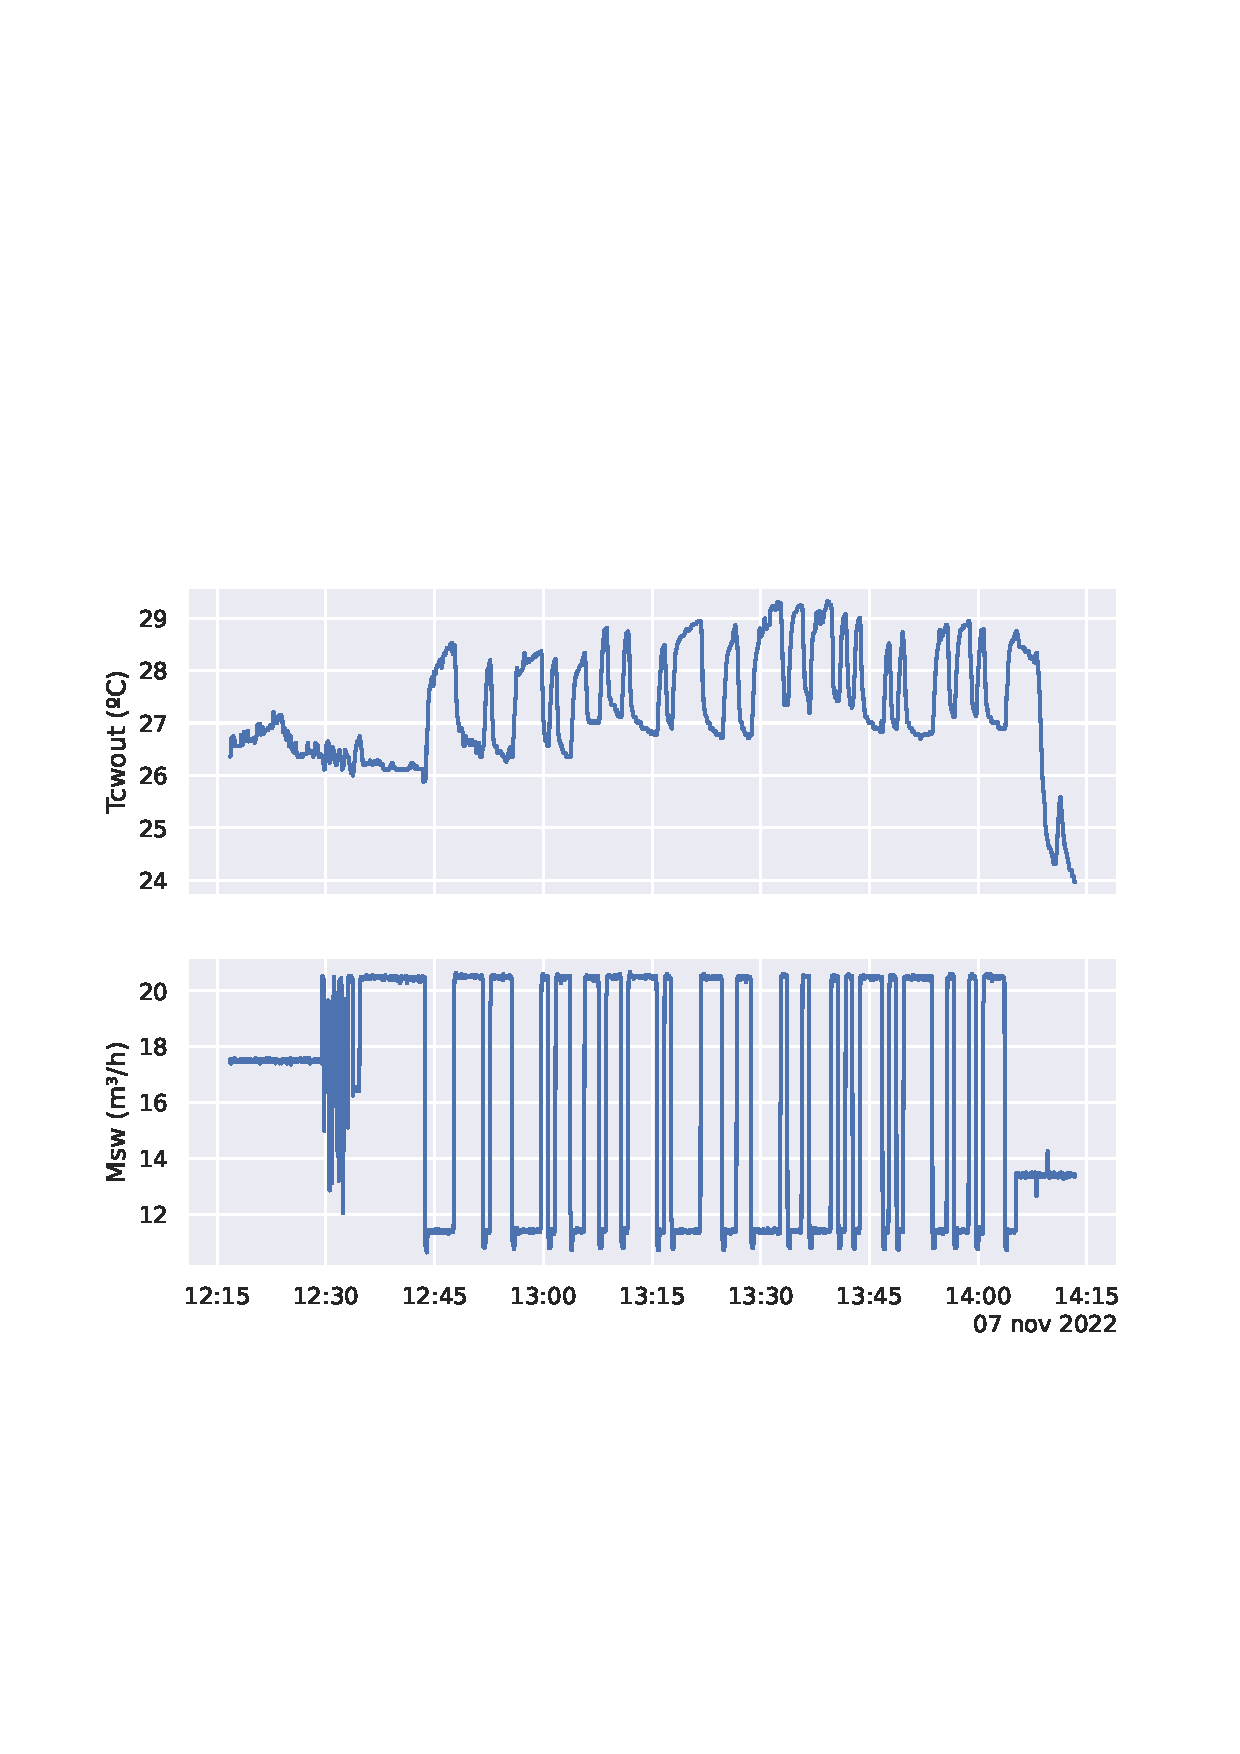
\includegraphics[width=0.48\linewidth]{solarmed-std-control-tcout-ident.png}
    }}%
    \hspace{0.1cm}
    \subfloat[\centering
    Controller application results]{{\includegraphics[width=0.48\linewidth]{solarmed-str-control-condenser_temperature.png}
    }}%
    \caption[Condenser outlet temperature controller implementation]{Condenser outlet temperature controller implementation. On (b) the perturbance (inlet temperature) is shown with a solid-green line, while the output (condenser outlet temperature) is shown with a solid-blue line. The reference is a thick dashed-green line.}
    \labfig{solarmed:std:condenser-control}
\end{figure*}

\subsubsection{Reproducibility and the effect of the steady state duration}
\labsec{solarmed:std:results:reproducibility}
% 20230331 12:15 and 20230418 12:22: Duration from 16 to 76
% 20230329 13:10 and 20230414 12:51: Also the same test on different dates

The operation points pairs 1--2 and 3--4 in \reftab{solarmed:std:results} are
the same test, \ie the same operating conditions, but performed on different
dates. Particularly for points 1--2, the duration of the steady state is
significantly different (16 and 76 minutes, respectively). The obtained
performance metrics are similar, with almost identical values for the energetic
(\gls{gorLabel}, \gls{stecLabel}) and separation metrics (\gls{rrLabel},
\gls{riLabel}). Minor differences, but still within the uncertainty margin are
observed in metrics influenced by electrical consumption ($\eta_{II}$,
\gls{sexcLabel}, \gls{seecLabel})---which varies between tests. The observed
differences are mainly due to variations in the cooling water inlet temperature,
which in turn affect the required cooling water flow rate. For point~1, the
inlet condenser temperature ($T_{c,in}$) is 24.5~$^\circ$C, requiring a cooling
water flow rate of 17~m$^3$/h ($J$=8.0\pm0.2~kW$_e$), whereas for point~2,
$T_{c,in}$ is 23~$^\circ$C, requiring 13~m$^3$/h ($J$=8.1\pm0.2~kW$_e$). These
differences result in a 0.3~\% variation in the second-law efficiency and
0.1~kWh$_e$/m$^3$ in the \gls{seecLabel}. In contrast, for points~3 and~4, the
inlet condenser temperatures are similar enough (22.6 and 21.4~$^\circ$C,
respectively), making the differences in all performance metrics negligible
($J$=8.1\pm0.2~kW$_e$ for both points).
 
% due to differences
% in the cooling water inlet temperature: 17 (1) \vs 13 (2) m$^3$/h for the
% cooling water flow rate, translates into a 0.3\% difference in second law
% efficiency and 0.1 KWh$_e$//m$^3$ for \gls{seecLabel}. Inlet condenser temperature
% conditions are more similar in 3--4 (22.6 vs 21.4~$^\circ$C), making differences
% for all metrics negligible.

Thus, it can be stated that the proposed methodology provides reproducible
results and that the quality of stable operation and the ability to correctly
identify it are of greater importance than the specific duration of the steady
state.


% Tabla medidas de 8 puntos de operación (2 alta T, 2 baja T, 2 control, 2 con diferente duración de estacionario)
% Tabla de métricas de 8 puntos de operación

\begin{table*}[]
\caption{Measured variables and performance metrics for some operation points of the experimental campaign. The values are expressed as mean $\pm$ standard deviation with a coverage factor of 2 (95\% confidence interval). \textit{D} is the duration of the steady state period.}
\labtab{solarmed:std:results}

\resizebox{.9\linewidth}{!}{%
\begin{tabular}{ccccccccccccccccccccc}
\hline
\multirow{2}{*}{} &  & \multirow{2}{*}{\begin{tabular}[c]{@{}c@{}}\textbf{Test date}\\ (UTC)\end{tabular}} &  & \multirow{2}{*}{\begin{tabular}[c]{@{}c@{}}\textbf{D}\\ (min)\end{tabular}} &  & \multicolumn{14}{c}{\textbf{Performance metrics}} \\ \cline{7-20}
           &  &                 &  &                           &  & \begin{tabular}[c]{@{}c@{}}GOR\\ {\footnotesize (-) }\end{tabular} &  & \begin{tabular}[c]{@{}c@{}}STEC\\ {\footnotesize ($KW_{th}/m^3$) }\end{tabular} &  & \begin{tabular}[c]{@{}c@{}}SEEC\\ {\footnotesize ($KW_{e}/m^3$) }\end{tabular} &  & \begin{tabular}[c]{@{}c@{}}RR\\ {\footnotesize (-) }\end{tabular} &  & \begin{tabular}[c]{@{}c@{}}RI\\ {\footnotesize (-) }\end{tabular} &  & \begin{tabular}[c]{@{}c@{}}$\eta_{II}$\\ {\footnotesize (\%) }\end{tabular} &  & \begin{tabular}[c]{@{}c@{}}SEXC\\ {\footnotesize ($kWh_{ex}/m^3$) }\end{tabular} \\ \cline{3-3} \cline{5-5}\cline{7-7} \cline{9-9} \cline{11-11} \cline{13-13} \cline{15-15} \cline{17-17} \cline{19-19}
1 &   & 20230331 12:15 &   & 16 &   & $11 \pm 1$ &   & $60 \pm 6$ &   & $3.9 \pm 0.2$ &   & $29 \pm 1$ &   & $0.35 \pm 0.02$ &   & $8.0 \pm 0.6$ &   & $10.9 \pm 0.8$ &   \\
2 &   & 20230418 12:22 &   & 76 &   & $11 \pm 1$ &   & $59 \pm 6$ &   & $4.0 \pm 0.2$ &   & $29 \pm 2$ &   & $0.35 \pm 0.02$ &   & $7.7 \pm 0.6$ &   & $11.3 \pm 0.9$ &   \\
\cline{3-20}
3 &   & 20230329 13:10 &   & 24 &   & $10.1 \pm 0.7$ &   & $66 \pm 5$ &   & $3.9 \pm 0.2$ &   & $30 \pm 2$ &   & $0.35 \pm 0.02$ &   & $6.9 \pm 0.4$ &   & $12.7 \pm 0.8$ &   \\
4 &   & 20230414 12:51 &   & 27 &   & $10.2 \pm 0.7$ &   & $65 \pm 5$ &   & $3.9 \pm 0.2$ &   & $30 \pm 2$ &   & $0.36 \pm 0.02$ &   & $6.8 \pm 0.4$ &   & $12.8 \pm 0.8$ &   \\
5 &   & 20230511 11:23 &   & 32 &   & $8.1 \pm 0.4$ &   & $81 \pm 4$ &   & $3.2 \pm 0.2$ &   & $44 \pm 2$ &   & $0.52 \pm 0.02$ &   & $4.6 \pm 0.3$ &   & $17.8 \pm 0.9$ &   \\
\cline{3-20}
6 &   & 20230414 11:49 &   & 18 &   & $11 \pm 1$ &   & $59 \pm 5$ &   & $3.8 \pm 0.2$ &   & $47 \pm 3$ &   & $0.56 \pm 0.03$ &   & $7.2 \pm 0.5$ &   & $11.9 \pm 0.9$ &   \\
7 &   & 20230508 11:00 &   & 54 &   & $7.0 \pm 0.4$ &   & $93 \pm 6$ &   & $3.7 \pm 0.2$ &   & $48 \pm 3$ &   & $0.57 \pm 0.03$ &   & $3.9 \pm 0.3$ &   & $21 \pm 1$ &   \\
\hline
\end{tabular}
}

\bigskip

% TODO: Actualizar tabla con separadores
% TODO: Quitar la columna wd
% TODO: STEC y SEEC unidades están bien

\resizebox{\linewidth}{!}{%
\centering
\begin{tabular}{ccccccccccccccccccccccccc}
\hline
\multirow{2}{*}{} &  & \multicolumn{22}{c}{\textbf{Measured variables}} \\ \cline{3-24}
           &  & \begin{tabular}[c]{@{}c@{}}$T_{s,in}$\\ {\footnotesize (\si{\degreeCelsius}) }\end{tabular} &  & \begin{tabular}[c]{@{}c@{}}$T_{c,out}$\\ {\footnotesize (\si{\degreeCelsius}) }\end{tabular} &  & \begin{tabular}[c]{@{}c@{}}$q_{s}$\\ {\footnotesize (\si{\liter\per\second}) }\end{tabular} &  & \begin{tabular}[c]{@{}c@{}}$q_{f}$\\ {\footnotesize (\si{\cubic\meter\per\hour}) }\end{tabular} &  & \begin{tabular}[c]{@{}c@{}}$q_{d}$\\ {\footnotesize (\si{\cubic\meter\per\hour}) }\end{tabular} &  & \begin{tabular}[c]{@{}c@{}}$T_{s,out}$\\ {\footnotesize (\si{\degreeCelsius}) }\end{tabular} &  & \begin{tabular}[c]{@{}c@{}}$T_{c,in}$\\ {\footnotesize (\si{\degreeCelsius}) }\end{tabular} &  & \begin{tabular}[c]{@{}c@{}}$w_{f}$\\ {\footnotesize (\si{\milli\siemens\per\centi\meter}) }\end{tabular} &  & \begin{tabular}[c]{@{}c@{}}$w_{d}$\\ {\footnotesize (\si{\micro\siemens\per\centi\meter}) }\end{tabular} &  & \begin{tabular}[c]{@{}c@{}}$q_{c}$\\ {\footnotesize (\si{\cubic\meter\per\hour}) }\end{tabular} &  & \begin{tabular}[c]{@{}c@{}}J\\ {\footnotesize (\si{\kilo\watt}) }\end{tabular} \\ \cline{3-3} \cline{5-5} \cline{7-7} \cline{9-9} \cline{11-11} \cline{13-13} \cline{15-15} \cline{17-17} \cline{19-19} \cline{21-21} \cline{23-23}
1 &   & $64.0 \pm 0.8$ &   & $28.1 \pm 0.6$ &   & $12.0 \pm 0.2$ &   & $8.0 \pm 0.1$ &   & $2.4 \pm 0.1$ &   & $61.1 \pm 0.7$ &   & $24.5 \pm 0.7$ &   & $67.4 \pm 0.7$ &   & $8.00 \pm 0.08$ &   & $17 \pm 1$ &   & $\left(8.0 \pm 0.2\right) \times 10^{3}$ &   \\
2 &   & $64.0 \pm 0.7$ &   & $28.0 \pm 0.6$ &   & $12.0 \pm 0.3$ &   & $8.0 \pm 0.1$ &   & $2.3 \pm 0.1$ &   & $61.2 \pm 0.7$ &   & $23 \pm 1$ &   & $67.4 \pm 0.7$ &   & $8.00 \pm 0.08$ &   & $13 \pm 2$ &   & $\left(8.1 \pm 0.2\right) \times 10^{3}$ &   \\
\cline{3-24}
3 &   & $68.0 \pm 0.7$ &   & $28.0 \pm 0.6$ &   & $12.0 \pm 0.2$ &   & $8.0 \pm 0.1$ &   & $2.4 \pm 0.1$ &   & $64.8 \pm 0.7$ &   & $22.6 \pm 0.6$ &   & $67.4 \pm 0.7$ &   & $8.00 \pm 0.08$ &   & $13.8 \pm 0.8$ &   & $\left(8.1 \pm 0.2\right) \times 10^{3}$ &   \\
4 &   & $68.0 \pm 0.7$ &   & $27.9 \pm 0.8$ &   & $12.0 \pm 0.3$ &   & $8.0 \pm 0.1$ &   & $2.4 \pm 0.1$ &   & $64.8 \pm 0.6$ &   & $21.4 \pm 0.8$ &   & $67.4 \pm 0.7$ &   & $8.00 \pm 0.08$ &   & $10.9 \pm 0.9$ &   & $\left(8.1 \pm 0.2\right) \times 10^{3}$ &   \\
5 &   & $88.9 \pm 0.9$ &   & $29 \pm 1$ &   & $12.0 \pm 0.3$ &   & $7.0 \pm 0.1$ &   & $3.1 \pm 0.1$ &   & $83.8 \pm 0.9$ &   & $22 \pm 1$ &   & $64.7 \pm 0.6$ &   & $8.00 \pm 0.08$ &   & $20.1 \pm 0.3$ &   & $\left(7.9 \pm 0.3\right) \times 10^{3}$ &   \\
\cline{3-24}
6 &   & $68.0 \pm 0.7$ &   & $28.0 \pm 0.5$ &   & $12.0 \pm 0.3$ &   & $5.0 \pm 0.1$ &   & $2.4 \pm 0.1$ &   & $65.2 \pm 0.7$ &   & $20.8 \pm 0.6$ &   & $67.4 \pm 0.7$ &   & $8.00 \pm 0.08$ &   & $10.1 \pm 0.4$ &   & $\left(7.9 \pm 0.3\right) \times 10^{3}$ &   \\
7 &   & $89.0 \pm 0.7$ &   & $28.1 \pm 0.6$ &   & $12.0 \pm 0.3$ &   & $5.0 \pm 0.1$ &   & $2.4 \pm 0.1$ &   & $84.4 \pm 0.8$ &   & $21 \pm 2$ &   & $64.5 \pm 0.7$ &   & $8.00 \pm 0.08$ &   & $16 \pm 3$ &   & $\left(7.8 \pm 0.3\right) \times 10^{3}$ &   \\
\hline
\end{tabular}
}

\end{table*}


% \begin{table*}[]
% \caption{Performance metrics for some operation points of the experimental campaign. The values are expressed as mean $\pm$ standard deviation with a coverage factor of 2 (95\% confidence interval). \textit{D} is the duration of the steady state period.}
% \labtab{solarmed:std:performance-metrics}
% \resizebox{\linewidth}{!}{%
% }
% \end{table*}

% %================================
% \subsection{Results analysis}

% When the system was planned, it was designed to optimize for \textit{seawater desalination} and considering \textit{process heat}\sidenote{See \refsec{solarmed:std:process}} as the only external thermal energy source. 

%This is reflected in the higher performance values that can be observed, with low temperature difference between inlet and outlet of the heat source, whereas for brine concentration low recoveries are observed, and poor performance values are observed for the waste heat metrics

% \subsubsection{Best operating strategy}

% One caveat of the exergetic metrics for this particular plant, where the sink\sidenote{the simulated-fixed volume seawater} can change its conditions with significant dynamics, is that otherwise similar operating points can have different exergetic performance due to the additional cooling consumption required to maintain a certain condenser pressure / condenser outlet temperature. In order to enable fair comparison of the exergetic performance of different operating points, the cooling consumption is normalized to seawater intake at 20~$^\circ$C. 

\subsubsection{Experimental evaluation at high \glsentrylongpl{tbtLabel}}

As mentioned in the introduction, in practice, the \gls{tbtLabel} in the
\gls{medLabel} system is typically limited to 70~$^\circ$C or below to prevent
scaling. This limitation can be assessed using the \gls{rsiLabel}, which
requires knowledge of the water pH. To obtain this parameter, a laboratory
analysis of the water composition was carried out for both the untreated seawater
at the intake of the \gls{medLabel} system and the pretreated water after the
nanofiltration unit. The results of this analysis are presented in
\reffig{solarmed:std:tbt-pretreatment} (center bar plot). Subsequently, the
\textit{PyEquIon} open-source library~\sidecite{marcellos_pyequion_2021} was
used to estimate the pH at various temperatures and concentration factors. For
the latter, it was assumed that all ions scale uniformly, \ie, that the
concentration factor is identical for all species. Based on these values, the
\gls{rsiLabel} was computed for different temperatures and concentrations.

For un-treated feedwater (\reffig{solarmed:std:tbt-pretreatment} - left) the
risk of precipitation is present at almost any temperature  due to its
composition\sidenote{\reffig{solarmed:std:tbt-pretreatment} -- \textit{seawater}
in center bar plot}. A nanofiltration
pretreatment\sidenote{\reffig{solarmed:std:tbt-pretreatment} --
\textit{pretreated water} in in center bar plot} is used to selectively remove
the divalent ions while leaving relatively unaffected the monovalent ones, \ie
NaCl. After pretreatment, severe scaling ---\gls{rsiLabel} values below 4--- can
only be observed above 80$^\circ$C and $\approx$ 100~g/kg as shown in
\reffig{solarmed:std:tbt-pretreatment} -- right.

\begin{figure*}[h!]
    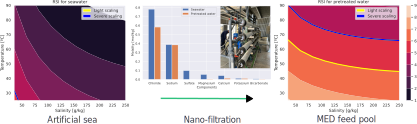
\includegraphics[]{solarmed-std-tbt-pretreatment.png}
    \caption{\gls{rsiLabel} values as a function of temperature and
    concentration before (left) and after (right) pretreatment using
    nanofiltration.}
    \labfig{solarmed:std:tbt-pretreatment}
\end{figure*}

Using a physical model of the plant\sidenote{A detailed description of the model
can be found in the Appendix, \nrefch{appendix:med-model}}, a better insight
into the inner working of the plant can be obtained. The model is based on the
energy and mass balances of the system, and it is used to estimate different
outputs at the effect level, such as the temperature and pressure of the vapor,
the distillate production, and the brine concentration.

\subsubsection{Scaling assessment during high \glsentrylong{tbtLabel} operation}

Using the aforementioned physical model of the plant, it is possible to analyze
the temperature and concentration evolution and visualize them as shown in
\reffig{solarmed:std:tbt-results}~(a). 

The figure shows the temperature and concentration evolution at each effect in
the \gls{medLabel} plant for several operation points: low-temperature operation
points (4:~68--8, 6:~68--5) and high-temperature operation points (5:~89--8,
7:~89--5). According to the \gls{rsiLabel}, the high-temperature operation
points (5,~7) enter the light scaling risk zone for the first seven effects
---above the yellow line in \reffig{solarmed:std:tbt-results}~(a)--- while the
low-temperature operation points (4,~6) remain within the stable water zone for
all effects.

To assess whether scaling occurred during high-temperature operation, control
tests were conducted both before the high-temperature tests and repeated after
approximately 30~hours of high \gls{tbtLabel} operation. In
\reftab{solarmed:std:results}, the same operation points used to validate
reproducibility\sidenote{\nrefsec{solarmed:std:results:reproducibility}}, \ie,
1--2 and 3--4, can be used to draw conclusions. No significant differences can
be observed for any of the performance indicators, with the values remaining
consistent between tests. This suggests that the system operated efficiently,
without significant fouling or scaling.

This is further confirmed by applying the physical model of the plant to
estimate the heat transfer coefficients. \reffig{solarmed:std:tbt-results}~(b)
illustrates the comparison of heat transfer coefficients before and after the
high-temperature campaign for both control tests. The results show only minor
variations between the pre- and post-high-temperature operation. With
measurements across all effects showing no systematic degradation trend. The
consistency of the coefficients indicates that no measurable scaling occurred
during the high \gls{tbtLabel} operation period.

\begin{figure*}
    \centering
    \subfloat[\centering Per effect temperature and concentration evolution. \\Surface represents the
    \gls{rsiLabel} for the pretreated feedwater.]{{\includegraphics[width=0.56\linewidth]{figures/solarmed-std-tbt-results.png}}}%
    \hspace{0.01\linewidth}
    \subfloat[\centering Heat transfer coefficients comparison]{{\includegraphics[width=0.42\linewidth]{figures/med-tbt-heat-tr-comp.png}}}%
    \caption{Scaling assessment during high \gls{tbtLabel} operation}
    \labfig{solarmed:std:tbt-results}
\end{figure*}

\subsubsection{Performance analysis at high \glsentrylong{tbtLabel}}

In \reftab{solarmed:std:results} operation points 4--5 and 6--7 compare low and
high \gls{tbtLabel} operation. Two of them (4 and 6) receive heat at
68$^\circ$C, while they differ in the feedwater flow rate ($q_f$), one (4) with
a higher value (8 m$^3$/h) and the other (6) at a lower one (5~m$^3$/h). The
other two operation points receive heat at 89$^\circ$C and similar feedwater
flow rate\sidenote{Equal between 4 and 5, slightly different but comparable
between 6 and 7}. The first two operation points result in an approximate
\gls{tbtLabel} of 61.5$^\circ$C while the last two operation points have an
approximate \gls{tbtLabel} of 79.2$^\circ$C. This operation points selection is
made to compare the performance of the plant at low and high \gls{tbtLabel}
operation with otherwise equivalent conditions.

The first key observation is that, contrary to the statement in the
introduction, the plant's performance does not improve with higher heat source
temperatures; rather, it deteriorates significantly. The \gls{gorLabel}
decreases by approximately 20\% and 36\% for the low (4--5) and high (6--7) \(
q_f \) scenarios, respectively. The results are even more pronounced in terms of
second-law efficiency, with reductions of 32\% and 46\%, respectively. This
decline occurs because higher-quality exergy is being destroyed in the
process. More energy ---of superior quality--- is being consumed to
produce distillate less efficiently\todo{comprobar números}.

This behavior is expected and can be attributed to the fact that the increase in
heat source temperature is not utilized to incorporate additional effects, which
would be the driver enhancing system efficiency.

On the other hand, the concentration achieved does increase significantly for
the high $q_f$ scenario, with a 47\% increase in the recovery ratio. This is not
the case for the low $q_f$ scenario, where the recovery ratio is similar to the
low temperature operation point. A possible explanation is presented
hereinafter.



% \begin{figure}
%     \includegraphics[width=.8\textwidth]{solarmed-std-tbt-results.png}
%     \caption{Temperature and concentration evolution for operation points at
%     each effect in the \gls{medLabel} plant. Surface represents the
%     \gls{rsiLabel} for the pretreated feedwater.}
%     \labfig{solarmed:std:tbt-results}
% \end{figure}

\begin{figure*}[h!]
    \savebox\captionqrleft{\qrcode[hyperlink,height=0.5in]{\repositoryBaseUrl/figures/med-tbt-energy-comp-68_28_12_5-20230414_vs_89_28_12_5-20230508.html}}
    \savebox\captionqrright{\qrcode[hyperlink,height=0.5in]{\repositoryBaseUrl/figures/med-tbt-vap-gen-comp-68_28_12_5-20230414_vs_89_28_12_5-20230508.html}}

    \subfloat[\centering
    Energy contribution. Number in brine bar represents percentage of energy absorbed by it]{{\includegraphics[width=0.48\linewidth]{med-tbt-energy-comp-68_28_12_5-20230414_vs_89_28_12_5-20230508.png}
    }}%
    \hspace{0.1cm}
    \subfloat[\centering
    Vapor generated. Value in bar represents flashing percentage]{{\includegraphics[width=0.48\linewidth]{med-tbt-vap-gen-comp-68_28_12_5-20230414_vs_89_28_12_5-20230508.png}
    }}%
    \caption{Per effect comparison between low and high \gls{tbtLabel} operation points\hfill \usebox\captionqrleft\hspace{1ex}\usebox\captionqrright}
    \labfig{solarmed:std:tbt-analysis}
\end{figure*}

A per effect comparison can also be made in terms of energy contribution for
vapor generation. This is shown in \reffig{solarmed:std:tbt-analysis} in terms
of energy contributions (a) and vapor generation mechanisms (b) for the low
$q_f$ (=5~m$^3$/h) operation points. In \reffig{solarmed:std:tbt-analysis}~(a)
it can be seen how, in the first effect, the only contributor to vapor
generation is the external heat source (red bar). For the following effects,
most of the energy comes from the previous effect vapor (purple bar) with some
contribution at specific effects ---10, 13-- from distillate coming from
previous effects (yellow bar, \textit{mixer})\sidenote{This is achieved by
sacrificing the previous effects distillate (green bar) in some other effects}.
The only negative contributor (it absorbs heat instead of releasing it) is the
brine (gray bar), which is warmed up. Also in the plot is shown the vapor
temperature evolution.

\reffig{solarmed:std:tbt-analysis}~(b) shows the vapor generation per effect
deaggregated in terms of the different mechanisms: boiling (gray bars) and
flashing (yellow bars). Additionally, the \gls{bpeLabel} of the brine is shown
as dashed lines. In this plot, it can be seen how in general boiling is the main
driver for vapor generation. 

In the first effect a stark difference between low and high operation can be
seen, with almost double the power released by the external source, producing
almost double the vapor ---\reffig{solarmed:std:tbt-analysis}~(b). However
this difference is not maintained in the following effects, but an opposite
trend is observed. Effect 8 is the crossing point and from there on the low
temperature operation point produces more vapor. Another interesting comparison
is the \textit{mixer} energy contribution, the higher temperature of the
distillate produced in the first effects becomes a signficant contributor in the
later effects, with a greater impact compared to the low temperature operation.
Thus, distillate distribution is more effective when total plant temperature
differences are higher. 

A possible explanation as to why vapor generation seems limited and thus the
achieved concentration, can be that the \gls{bpeLabel} of the brine
---\reffig{solarmed:std:tbt-analysis}~(b)--- is a function of temperature and
concentration, increasing with the latter. This means that the temperature
difference between the brine and the vapor is reduced, which in turn reduces the
boiling driving force. In the visualized case, the final \gls{bpeLabel} value
for the low-temperature operation is reached by effect 9 of the high temperature
one. In an  \gls{medLabel}  plant, the vapor generated in the previous effect is
the driving force for the next effect ---\reffig{solarmed:std:tbt-analysis}~(a).
Low vapor production on one effect means a diminished force for heat transfer in
the next one, which in turn reduces the vapor production on that effect. It is
an exponential decay process. That is why despite the larger energy availability
in the first effects, the better balaced effects of the low temperature
operation turns out to ultimately produce similar levels of
separation~\sidecite{lienhardv_energy_2019}.

Also in this figure, it can be seen than flashing takes a more relevant role in
vapor generation in the latter effects of the high temperature alternative,
since it is not affected by \gls{bpeLabel} (8, 9 and 17\% of the total vapor
generated in effects 12, 13 and 14, respectively). This indicates that maybe
flashing is a good alternative to increase the vapor production in the latter
stages of a thermal brine concentrator plant. 

\begin{remark}
    A \gls{medLabel}-MSF hybrid could be a good alternative to increase the brine
    concentration in the last effects, where the vapor production is limited by
    the \gls{bpeLabel}. Another option worth exploring is variable geometry
    effects, in order to increase temperature differences and mantain vapor
    production at higher concentrations.
\end{remark}
